\begin{document}
\maketitle

\begin{frame}
  \titlepage
\end{frame}

\cleardoublepage

\tableofcontents

\cleardoublepage

\section{Introduction}

\begin{frame}{Can of Worms}
\begin{figure}[!ht]
\centering

\includegraphics[width=0.75\linewidth]{img/canofworms.png}
\end{figure}
\end{frame}

\begin{frame}{Best Thing Since Sliced Bread}

% https://en.wikipedia.org/wiki/Sliced_bread#/media/File:Brood.jpg

\begin{figure}[!ht]
\centering
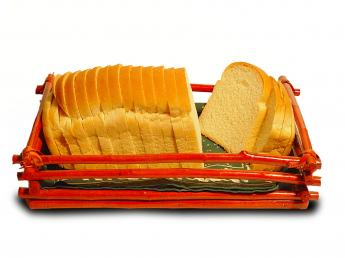
\includegraphics[width=1\linewidth]{img/sliced-bread.jpg}
\end{figure}
\end{frame}

\note{As you can imagine, the truth is in between these extremes}

\note{
  A few words about myself:
}

\begin{frame}{Me}
\begin{itemize}
\item Nick: racke
\item Selbstständiger Programmierer seit 1998
\item Webanwendungen
\item Ecommerce
\item Datendanken
\item Kunden in Österreich, Schweiz, USA, ...
\end{itemize}
\end{frame}

\note{
  One of my customers is the US Department of State.
  I'm responsible for a number of their web sites, for example
  the procurement solution eShop.
}

\begin{frame}{eShop}
\begin{figure}[!ht]
\centering
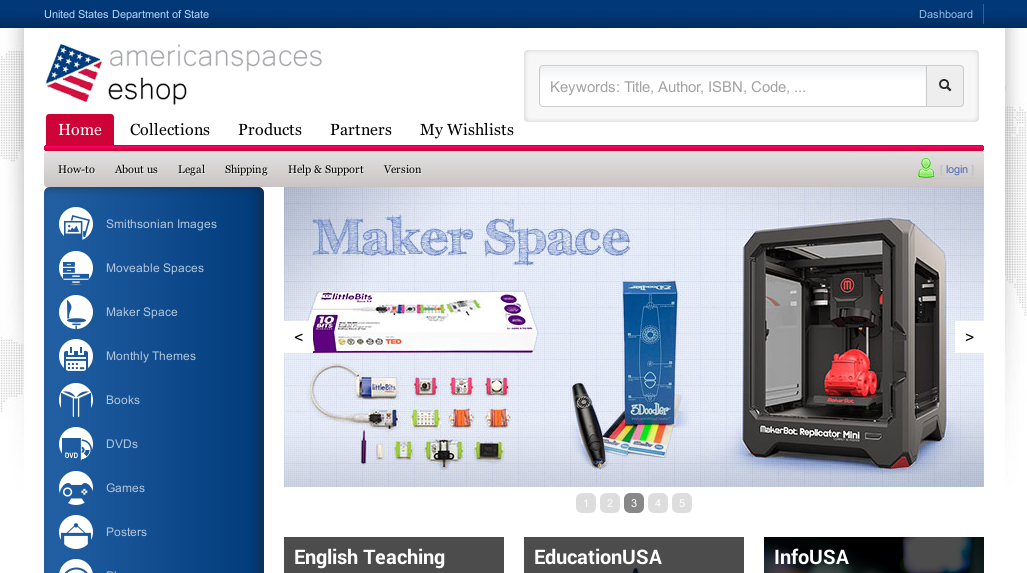
\includegraphics[width=1\linewidth]{img/eshop.png}
\end{figure}
\end{frame}

\begin{frame}{Interchange}
\begin{figure}[!ht]
\centering

\includegraphics[width=1\linewidth]{img/interchange.jpg}
\end{figure}
\end{frame}

\begin{frame}{Interchange}
\begin{itemize}
\item Embedded SQL
\item \sout{Modern Perl}
\end{itemize}
\end{frame}

\begin{frame}{Dancer / DBIx::Class}
\begin{itemize}
\item Dancer
\item DBIx::Class
\item Interchange6
\end{itemize}
\end{frame}

\note{We organized the second Perl Dancer conference October,}

\begin{frame}{Perl Dancer Conference}
\begin{figure}[!ht]
\centering

\includegraphics[width=1\linewidth]{img/perl-dancer-homepage-logo.png}
\end{figure}
\end{frame}

\note{where he had also a one day DBIx::Class training.

Here you see my co-trainers, ribasushi (mastermind behind
DBIx::Class) and Peter Mottram doing the last preparations
for the training:
}

\begin{frame}{DBIx::Class Training}
\begin{figure}[!ht]
\centering
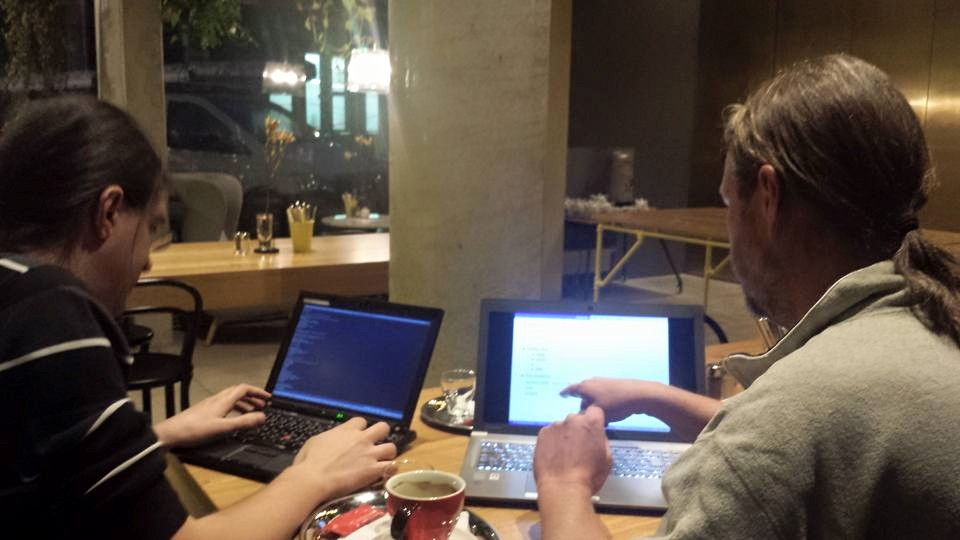
\includegraphics[width=1\linewidth]{img/training-preps.jpg}
\end{figure}
\end{frame}

\note{Baltimore Outage April}

\begin{frame}[fragile]{Conference website}
\begin{itemize}
\item ACT 2014
\begin{itemize}
\item Legacy code
\item No server control
\end{itemize}
\item www.perl.dance 2015
\begin{itemize}
\item Dancer / DBIx::Class
\item Most ACT features + new features
\item \url{https://github.com/interchange/Perl-Dancer-Conference}
\end{itemize}
\end{itemize}
\end{frame}

\subsection{Best Thing Since Sliced Bread}

\begin{frame}{Best Thing Since Sliced Bread}

% https://en.wikipedia.org/wiki/Sliced_bread#/media/File:Brood.jpg

\begin{figure}[!ht]
\centering
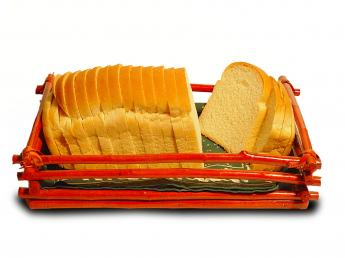
\includegraphics[width=1\linewidth]{img/sliced-bread.jpg}
\end{figure}
\end{frame}

\begin{frame}{Best Thing Since Sliced Bread}
\begin{itemize}
\item OO instead of SQL
\item Abstracts different SQL implementations
\item Businesslogik
\item Performance
\item ``ResultSet'' features
\item Ökosystem
\begin{itemize}
\item IRC / Mailing list
\item Komponenten
\item Helpers
\end{itemize}
\end{itemize}
\end{frame}

\subsection{Can of Worms}

\begin{frame}{Can of Worms}
\begin{figure}[!ht]
\centering

\includegraphics[width=0.75\linewidth]{img/canofworms.png}
\end{figure}
\end{frame}

DBIx::Class verwendet
\href{https://metacpan.org/pod/Class::C3::Componentised}{C3}.

\begin{frame}{Can of Worms}

\begin{itemize}
\item SQL::Abstract
\item Klassennamen (Result, ResultSet)
\item Basiert auf C3 anstatt Moo(se)
\item Dokumentation beschränkt auf DBIx::Class
\end{itemize}
\end{frame}

Using DBIx::Class allows you move all your business logic
into the database schema instead scattering it around a (web)
application.

\subsection{Businesslogik}
\begin{frame}{Businesslogik}
% move business logic into schema
% https://pixabay.com/en/gear-gears-euro-forex-dollar-384743/
\begin{figure}[!ht]
\centering

\includegraphics[width=0.75\linewidth]{img/business-logic.jpg}
\end{figure}
\end{frame}

\begin{frame}{Vorteile Businesslogik}
\begin{itemize}
\item Mehrere Verbraucher
\begin{itemize}
\item Webanwendungen
\item Cronjobs, Skripte
\item Testumgebungen
\end{itemize}
\item Implementation verbergen
\begin{itemize}
\item SQL-Dialekte
\item Anwendungsansicht
\end{itemize}
\item Änderungen / DRY
\end{itemize}
\end{frame}

\begin{frame}{Beispiele Businesslogik}
\begin{itemize}
\item Preisberechnungen
\begin{itemize}
\item Angebote
\item Rabatt
\end{itemize}
\item Synchronisierung ERP
\end{itemize}
\end{frame}

\subsection{Performance}

All the experience, tests and different areas in which 
DBIx::Class is applied makes it perform better than
handwritten SQL is most cases.

\begin{frame}{Performance}
\begin{itemize}
\item Erfahrung
\item Testsuiten
\item Use cases
\end{itemize}
\end{frame}
 
In case you feel that isn't correct, please call our hotline:

\begin{frame}{Hotline}
\begin{figure}[!ht]
\centering
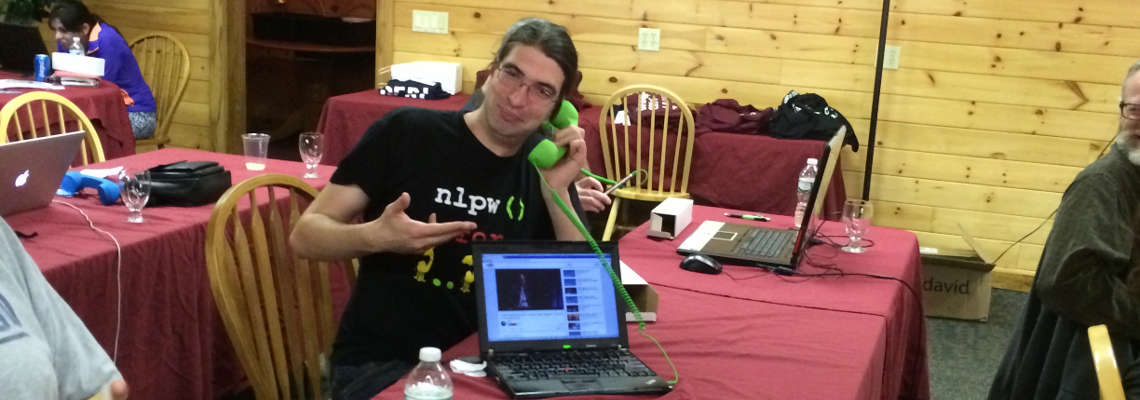
\includegraphics[width=1\linewidth]{img/perldance-2014-modern-tech.jpg}
\end{figure}
\end{frame}

But if you want to resort to SQL at some point, DBIx::Class allows you
to that too

\begin{frame}[fragile]{Literal SQL}
\begin{lstlisting}
$schema->resultset('PlaceVisited')->search(
{
  users_id => {
    -in => \[
       'SELECT users_id FROM users WHERE users_id > ?',
       2
    ]
  }
});
\end{lstlisting}
\end{frame}

But please don't complain if that leads to headache
and wasted time better spent on proper DBIx::Class
code.

\begin{frame}{SQL Kopfschmerzen}
% https://pixabay.com/en/stress-man-hand-flame-burn-fire-864141/
\begin{figure}[!ht]
\centering
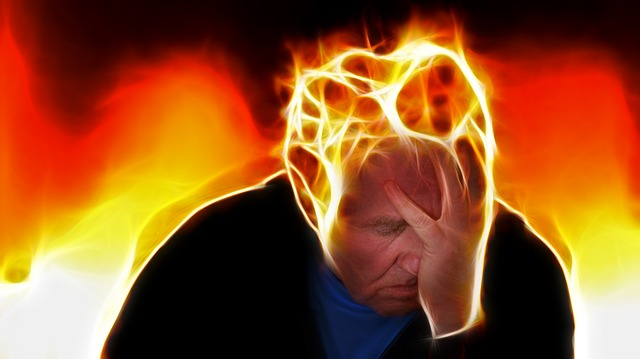
\includegraphics[width=1\linewidth]{img/stress.jpg}
\end{figure}
\end{frame}

\section{DBIx::Class Mengenlehre}

\note{The most important feature of DBIx::Class is the Resultset,
which we will examine through an example soon.}

\begin{frame}{DBIx::Class Mengenlehre}
\begin{itemize}
\item ORM
\begin{itemize}
\item Objects
\item Abstracts SQL
\item ...
\end{itemize}
\item ResultSet
\begin{itemize}
\item Verkettung
\item Relationship Traversal
\item Subqueries
\item ...
\end{itemize}
\end{itemize}
\end{frame}

\begin{frame}{Using ResultSet}
\begin{itemize}
\item Simple SQL query
\item Turn into DBIx::Class search
\item Use ResultSet features
\end{itemize}
\end{frame}

\begin{frame}[fragile]{Simple SQL query}
List of talks on last day of Perl Dancer Conference:
\begin{lstlisting}
SELECT talks_id, author_id, conferences_id, duration,
title, tags, abstract, url, comments, accepted, confirmed, 
lightning, scheduled, start_time, room, survey_id 
FROM talks 
WHERE accepted is TRUE 
AND conferences_id = 1 
AND room != '' 
AND start_time >= '2015-10-22 00:00:00'
AND start_time <= '2015-10-23 00:00:00'
\end{lstlisting}
\end{frame}

\begin{frame}[fragile]{Simple SQL query}
With DBIx::Class:
\begin{lstlisting}
my $talks = $schema->resultset('Talk')->search(
    {
        -bool          => 'accepted',
        conferences_id => 1,
        room           => { '!=' => '' },
        start_time     => {
            '>=' => '2015-10-22 00:00:00'
            '<=' => '2015-10-23 00:00:00'
            },
    },
);
\end{lstlisting}
\end{frame}

\subsection{Wahrheit über das ResultSet}
\note{
  If you hear the term ResultSet, you probably thing
  we are talking about a number of results aka
  table rows.
}

\begin{frame}{Wahrheit über das ResultSet}
\begin{figure}[!ht]
\centering
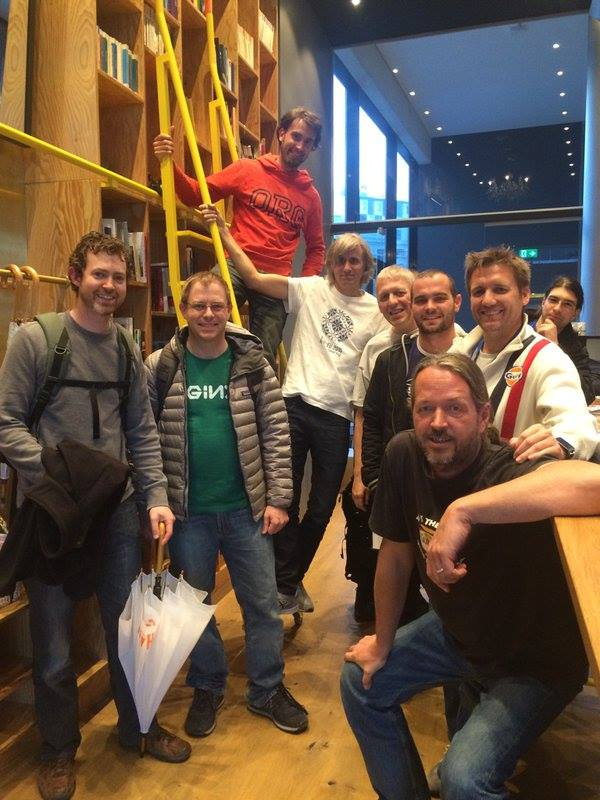
\includegraphics[width=0.5\linewidth]{img/pdc_users.jpg}
\end{figure}
\end{frame}

% https://pixabay.com/en/wrong-way-sign-road-caution-167535/

\begin{frame}{}
\begin{figure}[!ht]
\centering

\includegraphics[width=1\linewidth]{img/wrong-way.jpg}
\end{figure}
\end{frame}

\begin{frame}[fragile]{Wahrheit über das ResultSet}
% \centering
\sout{ResultSet}

\begin{lstlisting}
isa(Abfrageplan);
\end{lstlisting}

\end{frame}

\begin{frame}[fragile]{Wahrheit über das ResultSet}

Hier wird keine SQL-Abfrage ausgeführt:

\begin{lstlisting}
my $talks = $schema->resultset('Talk')->search(...);
\end{lstlisting}

Hier schon:

\begin{lstlisting}
my $first_talk = $schema->resultset('Talk')
                 ->search(...)->first;
\end{lstlisting}

\end{frame}

\section{ResultSet-Baukasten}

Composability means that you don't need to construct the
complete at once, but compose it together, e.g with
chaining.

The underlying mechanism is that \verb|->search| on a
ResultSet actually doesn't search.

% https://pixabay.com/en/regulation-screw-colorful-color-261927/

\begin{frame}{ResultSet-Baukasten}
\begin{figure}[!ht]
\centering
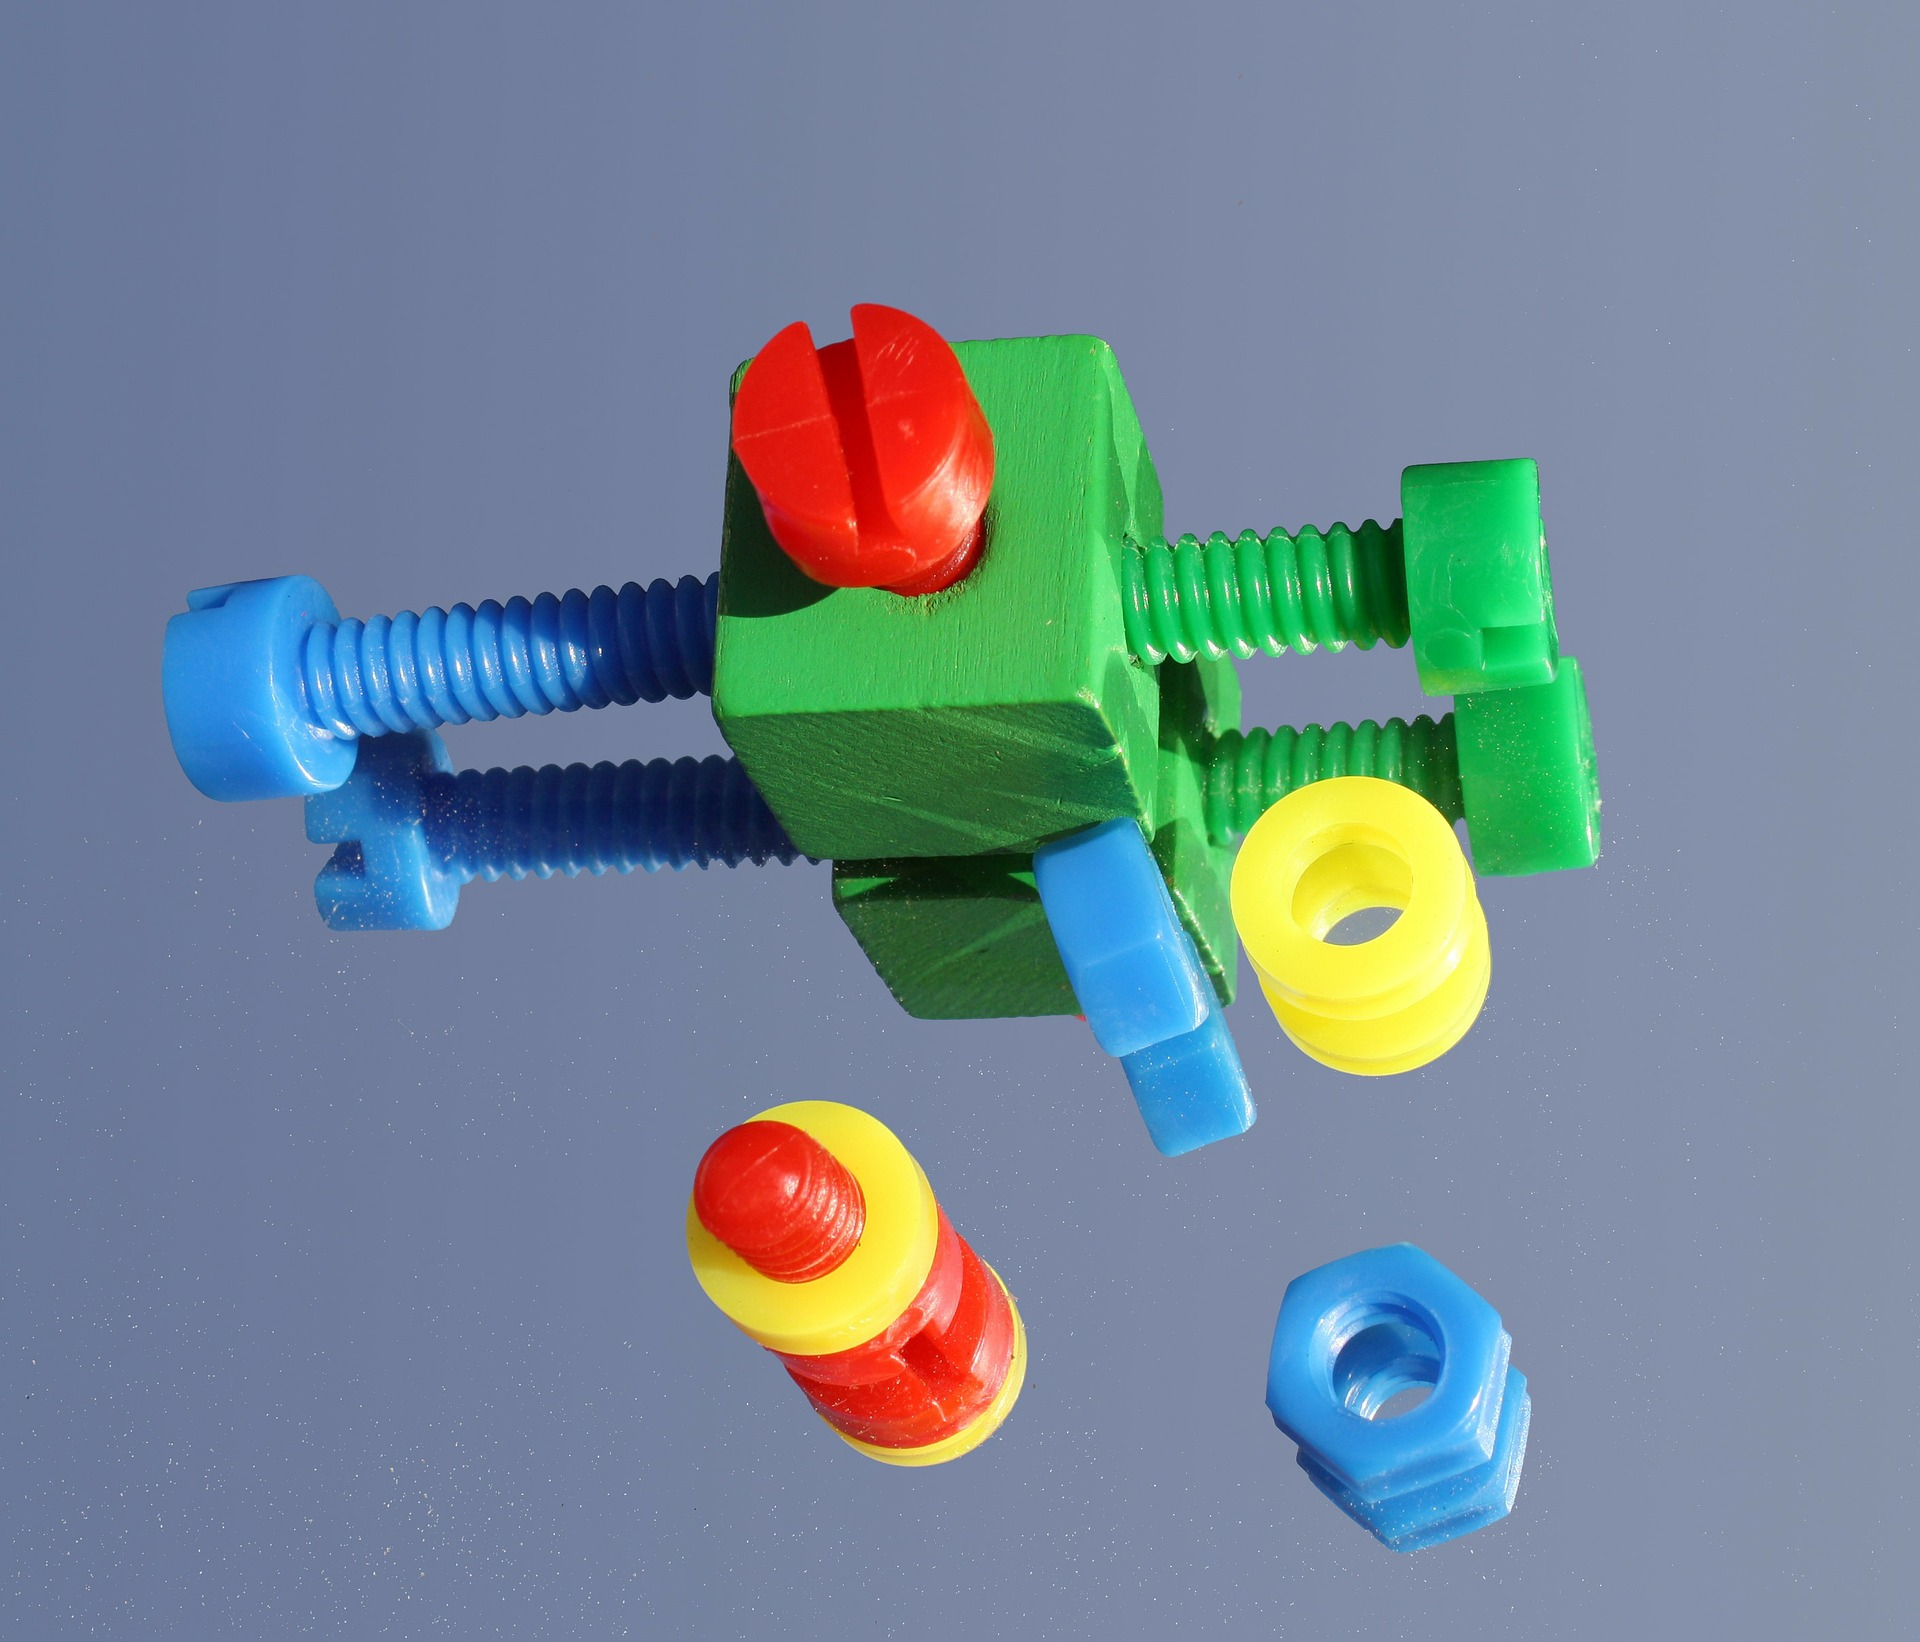
\includegraphics[width=0.70\linewidth]{img/baukasten.jpg}
\end{figure}
\end{frame}

\subsection{Verkettung}

\subsubsection{Suche ohne Verkettung}

\begin{frame}[fragile]{Suche ohne Verkettung}
\begin{lstlisting}
$schema->resultset('Product')->search({
    active => 1,
    canonical_sku => undef,
});
\end{lstlisting}
\end{frame}

\subsubsection{Suche mit Verkettung}

\begin{frame}[fragile]{Suche mit Verkettung}
\begin{lstlisting}
$schema->resultset('Product')->search({
    active => 1,
})->search({
    canonical_sku => undef,
});
\end{lstlisting}
\end{frame}

\subsubsection{Verkettung mit Update}

Die Verkettung kann auch genutzt werden, um
ein Suchergebnis mit einer anderen Operation zu
verknüpfen, z.B. ein \verb|UPDATE|.

\begin{frame}[fragile]{Verkettung mit Update}
\begin{lstlisting}
$schema->resultset('Product')->search({
    manufacturer => 'Out of Fashion',
})->update({
    active => 0,
});
\end{lstlisting}
\end{frame}

\subsection{Vordefinierte Suche}

\begin{frame}[fragile]{Vordefinierte Suche}
\begin{lstlisting}
package Interchange6::Schema::ResultSet::Product;

sub active {
    my $self = shift;

    return $self->search({ $self->me('active') => 1 });
}

sub canonical_only {
    my $self = shift;

    return $self->search({ 
       $self->me('canonical_sku') => undef });
}

\end{lstlisting}
\end{frame}

\subsubsection{Vordefinierte Suche anwenden}

\begin{frame}[fragile]{Vordefinierte Suche anwenden}
\begin{lstlisting}
$schema->resultset('Product')->active->canonical_only;
\end{lstlisting}
\end{frame}

\begin{frame}[fragile]{Vordefinierte Suche: Produktvarianten}
\begin{lstlisting}
sub with_variant_count {
 my $self = shift;
 return $self->search(
  undef,
  {
   '+columns' => {
     variant_count =>
      $self->correlate('variants')->count_rs->as_query
   }
  }
 );
}
\end{lstlisting}
\end{frame}

\subsection{Custom join conditions}

\begin{frame}[fragile]{Custom join conditions}
\begin{lstlisting}

__PACKAGE__->has_many(
  "addresses",
  "CalevoMobile::Schema::Result::Address",
  { "foreign.username" => "self.username" },
  { cascade_copy => 0, cascade_delete => 0 },
);

\end{lstlisting}
\end{frame}

\begin{frame}[fragile]{Custom join conditions}
\begin{lstlisting}

__PACKAGE__->has_many(
    "shipping_addresses",
    "CalevoMobile::Schema::Result::Address",
    sub {
        my $args = shift;

        return {
            "$args->{foreign_alias}.username" =>
                { -ident => "$args->{self_alias}.username",},
            "$args->{foreign_alias}.type" => 'shipping',
            "$args->{foreign_alias}.archived" => 0,
        }
    },
    { cascade_copy => 0, cascade_delete => 0 },
);
\end{lstlisting}
\end{frame}

\begin{frame}[fragile]{Subjects included}
\begin{itemize}
\item Me Helper
\verb|$self->me('active') => 1|
\end{itemize}
\end{frame}

\section{Erweiterungen}

\begin{frame}{Erweiterungen}
\begin{itemize}
\note{Zucker für DBIx::Class}
\item Candy
\item Subclassing Schema
\item Zusatzattribute
\item Komponenten
\item Helpers
\item Deployment Handler
\end{itemize}
\end{frame}

\subsection{Candy - Sugar for DBIx::Class}

\begin{frame}{Sugar for DBIx::Class}
% https://pixabay.com/en/candy-cane-candy-cane-winter-488009/
\begin{figure}[!ht]
\centering

\includegraphics[width=0.8\linewidth]{img/candy-cane.jpg}
\end{figure}
\end{frame}

\begin{frame}[fragile]{Vanilla Result Class}
\begin{lstlisting}
package TravelDance::Schema::Result::Country;
use warnings;
use strict;
use base 'DBIx::Class::Core';

__PACKAGE__->table('countries');

__PACKAGE__->add_columns(
    country_iso_code => {
        data_type => "char",
        size      => 2,
    },
    name => {
        data_type => "varchar",
        size      => 255,
    },
);
\end{lstlisting}
\end{frame}

\begin{frame}[fragile]{Candy Result Class}
\begin{lstlisting}
package TravelDance::Schema::Result::Country;
use TravelDance::Schema::Candy;

primary_column country_iso_code => {
    data_type => "char",
    size      => 2
};

column name => {
    data_type => "varchar",
    size      => 255
};
\end{lstlisting}
\end{frame}

\subsection{Subclassing Schemas}

\begin{frame}[fragile]{Use cases for subclassing}
\begin{itemize}
\item Generic schema e.g. \verb|Interchange6::Schema|
\item Applications with similar databases
\end{itemize}
\end{frame}

\begin{frame}{Subclassing}
\begin{itemize}
\item Tabellen hinzufügen
\item Spalten hinzufügen
\item Beziehungen hinzufügen
\end{itemize}
\end{frame}

\begin{frame}[fragile]{Subclass Beispiel}
\begin{lstlisting}
package PerlDance::Schema;
our $VERSION = 16;

use Interchange6::Schema::Result::User;
package Interchange6::Schema::Result::User;

__PACKAGE__->add_columns(
    bio => { data_type => "varchar", size => 2048, 
             default_value => '' },
    media_id =>
      { data_type => "integer", is_nullable => 1 },
    pause_id => { data_type => "varchar", size => 128, 
        default_value => '' },
    t_shirt_size => { data_type => "varchar", size => 8, 
      is_nullable => 1 },
);
\end{lstlisting}
\end{frame}

Inherit from \verb|Interchange6::Schema| and set result namespace to 
\verb|Interchange6::Schema::Result| plus \verb|PerlDance::Schema::Result|.

\begin{frame}[fragile]{Subclass Example}
\begin{lstlisting}
package PerlDance::Schema;

use base 'Interchange6::Schema';

Interchange6::Schema->load_namespaces(
    default_resultset_class => 'ResultSet',
    result_namespace        =>
        [ 'Result', '+PerlDance::Schema::Result' ],
    resultset_namespace     =>
        [ 'ResultSet', '+PerlDance::Schema::ResultSet' ],
);
\end{lstlisting}
\end{frame}

\subsection{Zusatzattribute für das Schema}

Für Funktionen der Businesslogik benötigen wir z.B.
Informationen über die Konfiguration der Webanwendung
bzw. den angemeldeten Benutzer.

\begin{frame}{Problemstellung}
\begin{itemize}
\item Konfiguration
\item angemeldeter Benutzer
\end{itemize}
\end{frame}

\begin{frame}[fragile]{Schemainstanz erzeugen}
\begin{lstlisting}
use Interchange6::Schema;

my $schema = Interchange6::Schema->connect(
  'dbi:Pg:dbname=perldance', 'racke', 'nevairbe', 
);
\end{lstlisting}
\end{frame}

\begin{frame}[fragile]{Zusatzattribute}
\begin{lstlisting}
__PACKAGE__->mk_group_ro_accessors(
    inherited => (
        [ 'current_user' => '_ic6_current_user' ]
    )
);

__PACKAGE__->mk_group_wo_accessors(
    inherited => (
        [ 'set_current_user' => '_ic6_current_user' ]
    )
);
\end{lstlisting}
\end{frame}

\begin{frame}[fragile]{Zusatzattribute}
\begin{lstlisting}
package Dancer::Plugin::Interchange6;

hook before => sub {
    shop_schema->set_current_user(
        logged_in_user || undef
    );
};

\end{lstlisting}
\end{frame}

\section{Komponenten}

Es gibt eine Vielzahl von Komponenten für DBIx::Class.

\subsection{Bäume}

Eine Baumstruktur, wie z.B. für die Navigation einer
Webseite, kann man mit Hilfe eines \verb|parent_id|-Feldes
darstellen.

\subsection{Tree::Adjacency Komponente}

\begin{frame}[fragile]{Tree::Adjacency Komponente}
\begin{lstlisting}

package Interchange6::Schema::Result::Navigation;

...

__PACKAGE__->load_components(qw( Tree::AdjacencyList ... ));

...

__PACKAGE__->add_columns(
   ...
 "parent_id",
  { data_type => "integer", default_value => 0, is_nullable => 0 },
   ...
);

...

__PACKAGE__->parent_column('parent_id');

\end{lstlisting}
\end{frame}

\begin{frame}{Tree::Adjacency Methoden}
\begin{itemize}
\item ancestors
\item children
\item siblings
\end{itemize}
\end{frame}

\section{DBIx::Class Helpers}

\begin{frame}{DBIx::Class Helpers}
Typische Anwendungsfälle für DBIx::Class vereinfachen.
\end{frame}

\begin{frame}{DBIx::Class Helpers}
\begin{figure}[!ht]
\centering

\includegraphics[width=0.4\linewidth]{img/frew.png}
\caption{Arthur Axel "fREW" Schmidt}
\end{figure}
\end{frame}

% list of helpers we show

\begin{frame}{DBIx::Class Helpers}
\begin{itemize}
\item Helper::Schema::QuoteNames
\item Helper::ResultSet::Me
\item Helper::Row::ProxyResultSetMethod
\item Helper::Row::OnColumnChange
\item Helper::Schema::DateTime
\end{itemize}
\end{frame}

\subsection{Helper::QuoteNames}

\begin{frame}[fragile]{Helper::QuoteNames}
\begin{itemize}
\item Maskierung von reservierten Wörtern
\item Änderungen zwischen Engines und Versionen
\item e.g. MySQL
\begin{itemize}
\item \verb|select user from userdb| => crash
\item \verb|select `user` from `userdb`| => works
\end{itemize}
\item \verb|quote_names| in connection info
\end{itemize}
\end{frame}

\begin{frame}[fragile]{Helper::QuoteNames}
\begin{lstlisting}

package Interchange6::Schema;

use base 'DBIx::Class::Schema';

__PACKAGE__->load_components( 
    'Helper::Schema::QuoteNames' 
);

...

\end{lstlisting}
\end{frame}

\subsection{Helper::ResultSet::Me}

Bei vordefinierten Suchen wissen wir nicht, welcher Tabellen-Alias
gebraucht wird.

Deshalb verwenden wir die \verb|current_source_alias|-Methode.

\begin{frame}[fragile]{Helper::Resultset::Me}
\begin{lstlisting}
sub active {
    my $self = shift;

    return $self->search({ 
        $self->current_source_alias . ".active" => 1,
    });
}
\end{lstlisting}
\end{frame}

Mit diesen Helper wird der Quellcode übersichtlicher:

\begin{frame}[fragile]{Helper::Resultset::Me}
\begin{lstlisting}
sub active {
    my $self = shift;

    return $self->search({ 
        $self->me('active') => 1,
    });
}
\end{lstlisting}
\end{frame}

\subsection{Helper::ResultSet::Shortcut}



\note{A lot of shortcuts are provided, I'll show
you just a few examples.}

\begin{frame}{Shortcuts}
\begin{itemize}
\item columns
\item like
\item hri
\end{itemize}
\end{frame}

\begin{frame}[fragile]{columns Shortcut}

\verb|columns| shortcut:

\begin{lstlisting}
$rs->columns([qw/ first_name last_name /]);
\end{lstlisting}

equivalent to:

\begin{lstlisting}
$rs->search( undef, { 
    columns => [qw/ first_name last_name /] 
} );
\end{lstlisting}
\end{frame}

\begin{frame}[fragile]{like Shortcut}

\verb|like| shortcut:

\begin{lstlisting}
$rs->like( 'city', 'region', '%York' );
\end{lstlisting}

or:

\begin{lstlisting}
$rs->like([ 'city', 'region' ], '%York' );
\end{lstlisting}

equivalent to:

\begin{lstlisting}
$rs->search(
    { city => { -like => '%York' },
    { region => { -like => '%York' },
);
\end{lstlisting}
\end{frame}

\subsection{HashRefInflator}

Using the HashRefInflator makes sense when you need to quickly retrieve
data from a massive resultset or you need a list of hash references anyway,
e.g. for input to a template in a web application.

\begin{frame}[fragile]{HashRefInflator}
\begin{lstlisting}
my $rs = $schema->resultset('Country')->search({}, {
   result_class
     => 'DBIx::Class::ResultClass::HashRefInflator',
 });
\end{lstlisting}
\end{frame}

\begin{frame}[fragile]{HashRefInflator mit HRI helper}
\begin{lstlisting}
my $rs = $schema->resultset('Country')->search({})->hri;

# since 'search' here is redundant we can just use:
my $rs = $schema->resultset('Country')->hri;
\end{lstlisting}
\end{frame}

\begin{frame}[fragile]{Tickets}
\begin{lstlisting}
 $tokens->{tickets} = [
    $schema->resultset('Conference')
        ->find( $conferences_id )
            ->tickets->active->prefetch('inventory')
                ->hri->all 
];
\end{lstlisting}
\end{frame}

\subsection{Helper::Row::ProxyResultSetMethod}

\begin{frame}[fragile]{Helper::Row::ProxyResultSetMethod}
\begin{lstlisting}
package Interchange6::Schema::Product;

use Interchange6::Schema::Candy -components => [
    qw( Helper::Row::ProxyResultSetMethod );
];

proxy_resultset_method 'variant_count';
\end{lstlisting}
\end{frame}

\subsection{Helper::Row::OnColumnChange}

\begin{frame}[fragile]{Helper::Row::OnColumnChange}

Do things when the value of a column changes.

\begin{itemize}
\item before\_column\_change
\item around\_column\_change
\item after\_column\_change
\end{itemize}

\end{frame}

\begin{frame}[fragile]{Helper::Row::OnColumnChange}

\begin{lstlisting}
package TravelDance::Schema::Result::User;

use TravelDance::Schema::Candy -components =>
    [qw(Helper::Row::OnColumnChange 
        InflateColumn::DateTime)];

use DateTime;

column last_password_change => {
    data_type => timestamp,
};
\end{lstlisting}
\end{frame}

\begin{frame}[fragile]{Helper::Row::OnColumnChange}

On password change:

\begin{itemize}
\item check new password against old one
\item update \verb|last_password_change| column
\end{itemize}

\end{frame}

\begin{frame}[fragile]{Helper::Row::OnColumnChange}
\begin{lstlisting}
after_column_change password => {
    method   => 'change_password',
    txn_wrap => 1,  # wrap it all in a transaction
};
\end{lstlisting}
\end{frame}

\begin{frame}[fragile]{Helper::Row::OnColumnChange}
\begin{lstlisting}
sub change_password {
    my ( $self, $old_value, $new_value ) = @_;
    if ( $self->check_password($new_value) ) {
        $self->throw_exception("Password not changed")
    }
    else {
        $self->update(
            { last_password_change => DateTime->now() }
        );
    }
}
\end{lstlisting}
\end{frame}

\subsection{Helper::Schema::DateTime}

\begin{frame}[fragile]{Helper::Schema::DateTime}

VisitedPlaces visited in the last year:

\begin{lstlisting}
my $dtf = $schema->storage->datetime_parser; # boilerplate
my $one_year_ago = $dtf->format_datetime(
    DateTime->now->subtract( year => 1 )
);

my $rs = $schema->resultset('PlaceVisited')->search(
    {
        visited => { '>' => $one_year_ago }
    }
);
\end{lstlisting}
\end{frame}

\begin{frame}[fragile]{Helper::Schema::DateTime}

With the helper:

\begin{lstlisting}
my $one_year_ago = $schema->format_datetime(
    DateTime->now->subtract( year => 1 )
);

my $rs = $schema->resultset('PlaceVisited')->search(
    {
        visited => { '>' => $one_year_ago }
    }
);
\end{lstlisting}
\end{frame}

\subsection{Other useful helpers}
\begin{frame}{Other Useful Helpers}
\begin{itemize}
\note{Easily correlate your ResultSets}
\item Helper::ResultSet::CorrelateRelationship
\note{Remove columns from search}
\item Helper::ResultSet::RemoveColumns
\note{Random results, don't use Helper::Random}
\item Helper::ResultSet::Random
\note{Force numeric context on numeric columns:}
\item Helper::Row::NumifyGet
\end{itemize}
\end{frame}

% \section{Writing Tests}
% \begin{frame}{Writing Tests}
% \end{frame}

\section{Schema \& Deployment}

\begin{frame}{Deployment}
\begin{itemize}
\item Generierung aus dem Schema
\item Generierung aus der Datenbank
\end{itemize}
\end{frame}

Es gibt aber auch Situationen, wo die
Generierung aus der Datenbank sinnvoll ist,
z.B. wenn man mit DBIx::Class beginnt und
bereits ein Schema für eine vorhandene
Datenbank benötigt.


\subsection{dbicdump}

You can use \verb|dbicdump| to create a ``boilerplate'' schema from the
existing database.

\begin{frame}[fragile]{dbicdump}
\begin{lstlisting}
dbicdump -o dump_directory=/home/dance/TravelDance/lib 
         TravelDance::Schema 
         dbi:Pg:dbname=perldance
\end{lstlisting}
\end{frame}

\subsection{Deploy/Upgrade/Downgrade}

\begin{frame}{Deployment Handler}
\begin{itemize}
\item DBIx::Class::DeploymentHandler
\item Datenbankänderungen einspielen
\item Datenbank upgraden
\item Datenbank downgraden
\end{itemize}
\end{frame}

\subsection{Skripte für Deployment Handler}
\begin{frame}{Skripte für Deployment Handler}
\begin{description}
\item[dh-prepare-version-storage] Installation Datenbanktabelle vorbereiten
\item[dh-install-version-storage] Installation Datenbanktabelle einspielen
\item[dh-prepare-upgrade] Upgrade vorbereiten
\item[dh-upgrade] Upgrade einspielen
\end{description}
\end{frame}

\subsection{Update Prinzipien}

\begin{frame}{Update Prinzipien}
\begin{itemize}
\item Backup anlegen
\item Schema ändern
\item Skripts hinzufügen
\item Bump version number
\item Upgrade vorbereiten
\item Upgrade einspielen
\end{itemize}
\end{frame}

Note: create backup can be done by DeploymentHandler itself.

\subsection{Schema ändern}

\begin{frame}{Schema ändern}
\begin{itemize}
\item Tabelle hinzufügen
\item Spalte hinzufügen
\item Spalte ändern
\end{itemize}
\end{frame}

\subsection{Bump version number}
\begin{frame}{Bump version number}
\begin{itemize}
\item Natural number => 1
\item Increase by 1 => 2
\end{itemize}
\end{frame}

\begin{frame}[fragile]{Version 1}
\begin{lstlisting}
package TravelDance::Schema;
use warnings;
use strict;
use base 'DBIx::Class::Schema';

our $VERSION = 1;

__PACKAGE__->load_namespaces();

1;
\end{lstlisting}
\end{frame}

\begin{frame}[fragile]{Version 2}
\begin{lstlisting}
package TravelDance::Schema;
use warnings;
use strict;
use base 'DBIx::Class::Schema';

our $VERSION = 2;

__PACKAGE__->load_namespaces();

1;
\end{lstlisting}
\end{frame}

\subsection{Prepare upgrade}

\begin{frame}[fragile]{Prepare upgrade}
\begin{lstlisting}
my $dh     = DBIx::Class::DeploymentHandler->new(
    {
        schema              => $schema,
        databases           => 'MySQL',
        sql_translator_args => { add_drop_table => 0 }
    }
);
$dh->prepare_deploy;
$dh->prepare_upgrade(
    {
        from_version => $dh->database_version,
        to_version => $dh->schema_version
    }
);
\end{lstlisting}
\end{frame}

\subsection{Add custom scripts}

\begin{frame}{Add custom scripts}
\begin{itemize}
\item Deployment
\item All upgrades
\item Specific upgrade
\end{itemize}
\end{frame}

\begin{frame}{Add custom scripts}
\begin{itemize}
\item Populate records on deployment
\item Add initial values for new tables
\begin{itemize}
\item hardcoded in script
\item from file
\end{itemize}
\end{itemize}
\end{frame}

\subsection{Internals}

Reference for directory layout:
\href{https://metacpan.org/pod/DBIx::Class::DeploymentHandler::DeployMethod::SQL::Translator}{DBIx::Class::DeploymentHandler::DeployMethod::SQL::Translator}

\begin{frame}[fragile]{Directories and files}
\begin{description}
\item[sql/PostgreSQL] SQL scripts for deploy and update
\item[sql/\_common] Custom scripts
\begin{description}
\item[sql/\_common/upgrade/\_any] All upgrades
\item[sql/\_common/upgrade/ 1-2] Upgrade from 1 to 2
\end{description}
\item[sql/\_deploy] Structure files (YAML)
\end{description}
\end{frame}

\section{Abschluß}

\begin{frame}{Abschluß}
\begin{itemize}
\item Resources
\item Slides
\item Fragen
\end{itemize}
\end{frame}

\subsection{Resources}
\begin{frame}[fragile]{Resources}
\begin{itemize}
\item Extensive Documentation
\begin{itemize}
\item \verb|DBIx::Class::Manual::*|
\item \verb|DBIx::Class::Manual::ResultClass|
\item \verb|DBIx::Class::ResultSet|
\item \verb|DBIx::Class::Relationship::*|
\end{itemize}
\item \href{http://www.perladvent.org/2012/2012-12-21.html}
{Perl Advent Calendar 2012: Set-based DBIx::Class}
by fRew
\end{itemize}
\end{frame}

\subsubsection{Interchange Resources}

\begin{frame}{Interchange Resources}
\begin{figure}[!ht]
\centering

\includegraphics[width=0.4\linewidth]{img/interchange6-logo-v2.png}
\end{figure}
\begin{itemize}
\item Interchange6::Schema
\item Demo Shop
\item Perl Dancer Conference
\end{itemize}
\end{frame}

\subsection{Slides}

\begin{frame}{Slides}
Slides:
\url{http://www.linuxia.de/talks/gpw2016/dbic-pr-de-beamer.pdf}
\end{frame}

\subsection{Fragen}

\begin{frame}{Fragen}
\centering
Fragen ?
\end{frame}

\end{document}

%%% Local Variables: 
%%% mode: latex
%%% TeX-master: t
%%% End: 
